% Options for packages loaded elsewhere
\PassOptionsToPackage{unicode}{hyperref}
\PassOptionsToPackage{hyphens}{url}
\PassOptionsToPackage{dvipsnames,svgnames,x11names}{xcolor}
%
\documentclass[
  letterpaper,
  DIV=11,
  numbers=noendperiod]{scrreprt}

\usepackage{amsmath,amssymb}
\usepackage{iftex}
\ifPDFTeX
  \usepackage[T1]{fontenc}
  \usepackage[utf8]{inputenc}
  \usepackage{textcomp} % provide euro and other symbols
\else % if luatex or xetex
  \usepackage{unicode-math}
  \defaultfontfeatures{Scale=MatchLowercase}
  \defaultfontfeatures[\rmfamily]{Ligatures=TeX,Scale=1}
\fi
\usepackage{lmodern}
\ifPDFTeX\else  
    % xetex/luatex font selection
\fi
% Use upquote if available, for straight quotes in verbatim environments
\IfFileExists{upquote.sty}{\usepackage{upquote}}{}
\IfFileExists{microtype.sty}{% use microtype if available
  \usepackage[]{microtype}
  \UseMicrotypeSet[protrusion]{basicmath} % disable protrusion for tt fonts
}{}
\makeatletter
\@ifundefined{KOMAClassName}{% if non-KOMA class
  \IfFileExists{parskip.sty}{%
    \usepackage{parskip}
  }{% else
    \setlength{\parindent}{0pt}
    \setlength{\parskip}{6pt plus 2pt minus 1pt}}
}{% if KOMA class
  \KOMAoptions{parskip=half}}
\makeatother
\usepackage{xcolor}
\setlength{\emergencystretch}{3em} % prevent overfull lines
\setcounter{secnumdepth}{5}
% Make \paragraph and \subparagraph free-standing
\ifx\paragraph\undefined\else
  \let\oldparagraph\paragraph
  \renewcommand{\paragraph}[1]{\oldparagraph{#1}\mbox{}}
\fi
\ifx\subparagraph\undefined\else
  \let\oldsubparagraph\subparagraph
  \renewcommand{\subparagraph}[1]{\oldsubparagraph{#1}\mbox{}}
\fi


\providecommand{\tightlist}{%
  \setlength{\itemsep}{0pt}\setlength{\parskip}{0pt}}\usepackage{longtable,booktabs,array}
\usepackage{calc} % for calculating minipage widths
% Correct order of tables after \paragraph or \subparagraph
\usepackage{etoolbox}
\makeatletter
\patchcmd\longtable{\par}{\if@noskipsec\mbox{}\fi\par}{}{}
\makeatother
% Allow footnotes in longtable head/foot
\IfFileExists{footnotehyper.sty}{\usepackage{footnotehyper}}{\usepackage{footnote}}
\makesavenoteenv{longtable}
\usepackage{graphicx}
\makeatletter
\def\maxwidth{\ifdim\Gin@nat@width>\linewidth\linewidth\else\Gin@nat@width\fi}
\def\maxheight{\ifdim\Gin@nat@height>\textheight\textheight\else\Gin@nat@height\fi}
\makeatother
% Scale images if necessary, so that they will not overflow the page
% margins by default, and it is still possible to overwrite the defaults
% using explicit options in \includegraphics[width, height, ...]{}
\setkeys{Gin}{width=\maxwidth,height=\maxheight,keepaspectratio}
% Set default figure placement to htbp
\makeatletter
\def\fps@figure{htbp}
\makeatother
% definitions for citeproc citations
\NewDocumentCommand\citeproctext{}{}
\NewDocumentCommand\citeproc{mm}{%
  \begingroup\def\citeproctext{#2}\cite{#1}\endgroup}
\makeatletter
 % allow citations to break across lines
 \let\@cite@ofmt\@firstofone
 % avoid brackets around text for \cite:
 \def\@biblabel#1{}
 \def\@cite#1#2{{#1\if@tempswa , #2\fi}}
\makeatother
\newlength{\cslhangindent}
\setlength{\cslhangindent}{1.5em}
\newlength{\csllabelwidth}
\setlength{\csllabelwidth}{3em}
\newenvironment{CSLReferences}[2] % #1 hanging-indent, #2 entry-spacing
 {\begin{list}{}{%
  \setlength{\itemindent}{0pt}
  \setlength{\leftmargin}{0pt}
  \setlength{\parsep}{0pt}
  % turn on hanging indent if param 1 is 1
  \ifodd #1
   \setlength{\leftmargin}{\cslhangindent}
   \setlength{\itemindent}{-1\cslhangindent}
  \fi
  % set entry spacing
  \setlength{\itemsep}{#2\baselineskip}}}
 {\end{list}}
\usepackage{calc}
\newcommand{\CSLBlock}[1]{\hfill\break\parbox[t]{\linewidth}{\strut\ignorespaces#1\strut}}
\newcommand{\CSLLeftMargin}[1]{\parbox[t]{\csllabelwidth}{\strut#1\strut}}
\newcommand{\CSLRightInline}[1]{\parbox[t]{\linewidth - \csllabelwidth}{\strut#1\strut}}
\newcommand{\CSLIndent}[1]{\hspace{\cslhangindent}#1}

\KOMAoption{captions}{tableheading}
\makeatletter
\@ifpackageloaded{tcolorbox}{}{\usepackage[skins,breakable]{tcolorbox}}
\@ifpackageloaded{fontawesome5}{}{\usepackage{fontawesome5}}
\definecolor{quarto-callout-color}{HTML}{909090}
\definecolor{quarto-callout-note-color}{HTML}{0758E5}
\definecolor{quarto-callout-important-color}{HTML}{CC1914}
\definecolor{quarto-callout-warning-color}{HTML}{EB9113}
\definecolor{quarto-callout-tip-color}{HTML}{00A047}
\definecolor{quarto-callout-caution-color}{HTML}{FC5300}
\definecolor{quarto-callout-color-frame}{HTML}{acacac}
\definecolor{quarto-callout-note-color-frame}{HTML}{4582ec}
\definecolor{quarto-callout-important-color-frame}{HTML}{d9534f}
\definecolor{quarto-callout-warning-color-frame}{HTML}{f0ad4e}
\definecolor{quarto-callout-tip-color-frame}{HTML}{02b875}
\definecolor{quarto-callout-caution-color-frame}{HTML}{fd7e14}
\makeatother
\makeatletter
\@ifpackageloaded{bookmark}{}{\usepackage{bookmark}}
\makeatother
\makeatletter
\@ifpackageloaded{caption}{}{\usepackage{caption}}
\AtBeginDocument{%
\ifdefined\contentsname
  \renewcommand*\contentsname{Table of contents}
\else
  \newcommand\contentsname{Table of contents}
\fi
\ifdefined\listfigurename
  \renewcommand*\listfigurename{List of Figures}
\else
  \newcommand\listfigurename{List of Figures}
\fi
\ifdefined\listtablename
  \renewcommand*\listtablename{List of Tables}
\else
  \newcommand\listtablename{List of Tables}
\fi
\ifdefined\figurename
  \renewcommand*\figurename{Figure}
\else
  \newcommand\figurename{Figure}
\fi
\ifdefined\tablename
  \renewcommand*\tablename{Table}
\else
  \newcommand\tablename{Table}
\fi
}
\@ifpackageloaded{float}{}{\usepackage{float}}
\floatstyle{ruled}
\@ifundefined{c@chapter}{\newfloat{codelisting}{h}{lop}}{\newfloat{codelisting}{h}{lop}[chapter]}
\floatname{codelisting}{Listing}
\newcommand*\listoflistings{\listof{codelisting}{List of Listings}}
\makeatother
\makeatletter
\makeatother
\makeatletter
\@ifpackageloaded{caption}{}{\usepackage{caption}}
\@ifpackageloaded{subcaption}{}{\usepackage{subcaption}}
\makeatother
\ifLuaTeX
  \usepackage{selnolig}  % disable illegal ligatures
\fi
\usepackage{bookmark}

\IfFileExists{xurl.sty}{\usepackage{xurl}}{} % add URL line breaks if available
\urlstyle{same} % disable monospaced font for URLs
\hypersetup{
  pdftitle={Flow mapping with Arabesque 2},
  pdfauthor={Françoise Bahoken},
  colorlinks=true,
  linkcolor={blue},
  filecolor={Maroon},
  citecolor={Blue},
  urlcolor={Blue},
  pdfcreator={LaTeX via pandoc}}

\title{Flow mapping with Arabesque 2}
\author{Françoise Bahoken}
\date{2024-06-04}

\begin{document}
\maketitle

\renewcommand*\contentsname{Table of contents}
{
\hypersetup{linkcolor=}
\setcounter{tocdepth}{2}
\tableofcontents
}
\bookmarksetup{startatroot}

\chapter*{Welcome}\label{welcome}
\addcontentsline{toc}{chapter}{Welcome}

\markboth{Welcome}{Welcome}

This is the \textbf{\emph{Flow mapping with Arabesque 2}} online home
book.

\emph{Arabesque} is part of the Free and Open Source Software for
Geospatial (FOSS4G) movement. It is a web application dedicated to flow
mapping from origin-destination matrices and spatial networks datasets.

This books presents the functionnalities and how \emph{Arabesque} 2 can
be used to draw flowmaps.

It will be progressively updated following \emph{Arabesque} 2 current
development.

\begin{itemize}
\tightlist
\item
  On ligne version of \emph{Arabesque} can be accessed here:
  \href{https://arabesque.univ-eiffel.fr/}{arabesque.univ-eiffel.fr}
\end{itemize}

\begin{itemize}
\tightlist
\item
  The development version (the most complete) can be accessed here:
  \href{https://tonhauck.github.io/dev-arabesque/}{./dev-arabesque}
\end{itemize}

This book is reproducible and generated in R with Quarto.\\
Feel free to help us make it better and report any issue on
\href{https://github.com/gflowiz/arabesque}{GitHub}.

\href{http://creativecommons.org/licenses/by-nc-sa/4.0/}{\includegraphics{index_files/mediabag/88x31.png}}\\
This work by the geographic flow vizualisation research team is licensed
under a
\href{http://creativecommons.org/licenses/by-nc-sa/4.0/}{Creative
Commons Attribution-NonCommercial-ShareAlike 4.0 International License}.

\href{https://github.com/gflowiz/arabesque2-doc}{
\includegraphics[width=0.41667in,height=\textheight]{images/github.png}}
View source

\bookmarksetup{startatroot}

\chapter{Preface}\label{preface}

This Quarto book contains the online documentation of the second version
of \href{arabesque.univ-eiffel.fr}{\emph{Arabesque}}, a web application
for thematic flow mapping created within the geographic flow
vizualisation research program
(\href{https://geoflowiz.hypotheses.org/accueil/abstract}{gflowiz})
funded by \href{www.univ-eiffel.fr}{Univ. Gustave Eiffel} (former
IFSTTAR).

\hfill\break
The gflowiz project was originally led by Françoise Bahoken and
co-directed by Étienne Côme (Univ. Gustave Eiffel), with the scientific
collaboration of Laurent Jégou (Univ. Toulouse 2 Jean Jaurès). The main
developer of the first version of \emph{Arabesque} was Thomas Bapaume
(ESIEE student engineer), then Paul Fabre (UGE/IGN student
geographer/geomatician) ; Tony Hauck (freelance geomatician) is
developping the \emph{Arabesque2} version. Other contributors include
for the conception \& design of the app : Marion Maisonobe and Grégoire
le Campion (CNRS), and t for the Arabesque 1 documentation : Nicolas
Roelandt (Univ. Gustave Eiffel).

\emph{Arabesque} is an innovative cartographic application that meets
the contemporary challenges of spatial networks geovisualisation.

\section{Challenges}\label{challenges}

The analysis of the dynamics of urban areas or metropolises in one hand,
the delimitation of their functional areas and the spatio-temporal
comparison of their patterns in the other hand, are often limited by two
categories of problems inherent in data and tools.\\
\strut \\
The lack of open origin-destination (OD) data sets depicting territorial
interactions and interrelations limited the possibility of empirical
analysis. Similarly, the lack of dedicated geovisualization and
cartographic analysis tools means that many images of visual and
analytical interest are no longer part of the current cartographic
landscape. In addition to these specific problems regarding online OD
data, it is important to focus attention on the current possibilities
offered by online possibilities of OD cartography.

The current range of possibilities for exploring flows and networks
datasets on the geoweb is symptomatic of the ongoing enthusiasm of a
growing interdisciplinary community. While for a long time the efforts
were limited to direct visualisation alone, applications specifically
dedicated to flows have recently come on line.

\section{State of the Art}\label{state-of-the-art}

Three development approaches seem to be coexisting. The first one seems
to be dedicated to the development of large volumes of data in a digital
cartographic form, as is the case with the United Nations
\href{https://comtrade.un.org/}{Comtrade} for example. The second
approach consists of applications for the visual geographical
exploration of one's own OD datasets as in
\href{https://flowmap.blue/}{flowmap.blue}, for example. Academic
applications offer different graphical models allowing co-visualization,
such as the
\href{https://networkcube.github.io/vistorian/index.html}{Vistorian}
(Serrano Molinero \& al., 2017) and
\href{https://www.irit.fr/netscity/}{Netscity} (Maisonobe \& al., 2019).
The third approach is specific to heavy online thematic mapping software
infrastructures such as \hyperref[0]{Magrit} or \hyperref[0]{Kepler} in
response to the shortcomings of current editors regarding flow mapping.
It is interesting to note that all these solutions are being developed
in line with the growing practice of open-source development with a view
to reproducibility (Giraud, Lambert, 2017).

Few applications, however, appear to be fully aligned with the
``visualization mapping'' paradigm as defined by A. Mac Eachren (2004).
Indeed, efforts still seem to be focused more on displaying layers and
simply exploring them. Existing tools still do little to combine within
a single interface the three pillars of cartographic representation:
(geo)visualization and the processing of statistical and geographic
data.

In this context, \emph{Arabesque's} objectives are as follows.

\section{Objectives}\label{objectives}

\emph{Arabesque's} ambition is to meet the high demand for analysis of
one's own flow dataset in a free, open source and ergonomic way - this
need corresponding to the main result of our survey conducted in 2018.\\
\strut \\
\emph{Arabesque} is part of the french Lemaire Law for a digital
republic. It falls under the general objective of increasing
understanding of the geographical determinants of the spatial mobility
of goods, people and so on.\\
\strut \\
\emph{Arabesque} aims to respond to the need to visualize the results of
fundamental or applied research within theoretical and methodological
development frameworks that can be considered both transverse to several
subjects (population, habitat, environment, transport, i.e.) and
interdisciplinary by nature (geography, demography, environment,
geomatics, engineering sciences, human and social sciences, i.e.). These
subjects also contribute to the societal challenges linked to the rise
of the digital society, which they help to address.

From a scientific point of view, \emph{Arabesque} aims to innovate in
the handling of flow and network data currently available on the geoweb
(Bahoken et al, 2020). This is why it is part of the Mac Eachren (2005)
new paradigm of ``visualization mapping''.\\
\emph{Arabesque} combines in the same environment geo-visualization and
geographic and statistical information processing devices - initially
for descriptive purposes. On the other hand, it enables the processing
of complex relational datasets, which can be both voluminous and display
different dimensions of spatial mobilities (several thematic categories
and/or temporalities).\\
Particular attention is paid to rendering, both in terms of drawing and
the cartographic semiology of linear features. The desire to improve the
quality of the images of flows produced should lead to the development
of a sensible approach to the geo-visualization of mobilities and
spatial interactions.

Françoise Bahoken and Étienne Côme

Paris, Mai 2024.

\textbf{Quoted references:}

Keim D., Andrienko G., Fekete J.-D., Görg C., Kohlhammer J., Melançon G.
(2008), \emph{Visual Analytics: Definition, Process, and Challenges},
In: Kerren A. \& al.~(Eds.): Information Visualization, Springer-Verlag
Berlin Heidelberg, LNCS 4950, pp.~154--175.

Mac Eachren A. (2005), \emph{How Maps Work. Representation,
Visualization, and Design, New-York, The Guildford Press.}

Maisonobe M., Jégou L., Yakimovich N., Cabanac G. (2019), NETSCITY: a
geospatial application to analyse and map world scale production and
collaboration data between cities, \emph{International Conference on
Scientometrics and Informetrics (ISSI 2019)}, sep. 2019, Rome, Italy,
\href{https://hal.science/hal-02301035}{〈hal-02301035〉}

Giraud T., Lambert N. (2017), Reproducible cartography, in:
\emph{Advances in Cartography and GISsciences}, International
Cartographic Conference, ICACI'2017, Springer, pp.173-183.

Serrano Molinero V., Bach B., Plaisant C., Dufournaud N.,Fekete J.-D.
(2017), Understanding the Use of The Vistorian: Complementing Logs with
Context Mini-Questionnaires, \emph{Visualization for the Digital
Humanities}, Oct.~2017, Phoenix, United States.
\href{https://inria.hal.science/hal-01650259}{⟨hal-01650259⟩}.

\bookmarksetup{startatroot}

\chapter{Introduction}\label{introduction}

\emph{Arabesque} is dedicated to origin-destination flow and network
datasets. This second version enables data to be explored, filtered,
geovisualised and represented. \emph{Arabesque} lets you create flow
maps from your own datasets, using a web browser running \emph{Mozilla},
\emph{Chrome} or \emph{Brave}. It is based on current technological
possibilities, in particular those offered by the new web visualization
and mapping libraries (\emph{openlayers, d3, OSM, Turf,
NaturalEarthData}).

\textbf{General keywords}: cartography, geovisualisation, matrice,
flows, networks

\section{Main steps}\label{main-steps}

There are 5 main stages in creating a flowmap with \emph{Arabesque}:

\begin{enumerate}
\def\labelenumi{\arabic{enumi}.}
\tightlist
\item
  Importing your flowdata sets (at least for weighted links)
\item
  Processing flow data (creation of indicators)
\item
  Data exploration and configuration

  \begin{enumerate}
  \def\labelenumii{\arabic{enumii}.}
  \tightlist
  \item
    Numerical filtering of data
  \item
    Dealing with geography layers or tiles
  \end{enumerate}
\item
  Graphical symbolization (geometry and semiology)
\item
  Exporting and saving the \emph{Arabesque} workspace
\end{enumerate}

\bookmarksetup{startatroot}

\chapter{Summary}\label{summary}

This is the \textbf{\emph{Flow mapping with Arabesque}} online home
book, a free and open Source Software web application funded by the
french Université Gustave Eiffel.

Arabesque is dedicated to flow and network mapping, from
origin-destination simple or complexes matrices. Arabesques allows users
to filter flow data sets (nodes, links and flow values), to play with
geographic context (add tiles), reprojecting geography and to
parameterise the semiology of the drawings.

Built in javascript and HTML 5, Arabesque provides a full toolset to
explore, filter and geovisualize your Origin-Destination matrices. It
allows also to build clearer and understandable flow maps that respect
the principles of contemporary cartographic semiology.

Arabesque 2 is currently under development. See
\href{https://github.com/gflowiz/arabesque-dev}{arabesque-dev github
repository}.

\textbf{Contacts} :
\href{mailto:francoise.bahoken@univ-eiffel.fr,etienne.come@univ-eiffel.fr}{Françoise
BAHOKEN \& Étienne CÔME}

\bookmarksetup{startatroot}

\chapter{Arabesque' interface}\label{arabesque-interface}

Arabesque interface is accessible via its general home page.

\section{Arabesque Home page}\label{arabesque-home-page}

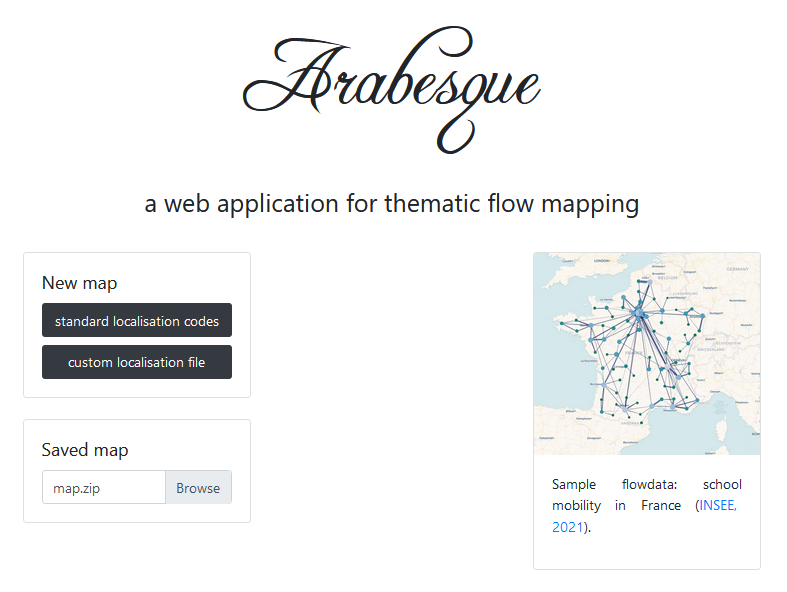
\includegraphics{images/Arabesque_homepage.png}

Through this home page, you can:

\begin{itemize}
\tightlist
\item
  Start a new flowmap by loading at least your flow data. See Data
  importation chapter.
\end{itemize}

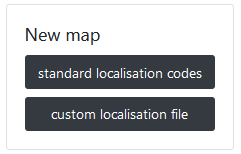
\includegraphics{images/Arabesque_homepage_newmap.png}

\begin{itemize}
\item
  Load a previous map via the Arabesque workspace

  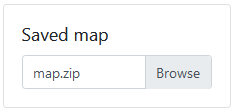
\includegraphics{images/Arabesque_homepage_savemap.png}
\item
  Load the example of school mobility flows (mobscol data set). See
  Examples for more information.

  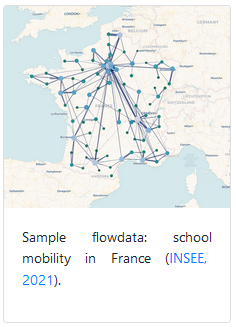
\includegraphics{images/Arabesque_homepage_sample.png}
\end{itemize}

\section{General structure}\label{general-structure}

\subsection{The main banner}\label{the-main-banner}


\includegraphics{images/main_banner.png}


\includegraphics{images/Buton_home.png} Return to
\href{https://arabesque.univ-eiffel.fr/}{the home page} to start a new
view.


\includegraphics{images/main_doc.png} Access to documentation


\includegraphics{images/main_about.png} Access to credits

\href{https://www.univ-gustave-eiffel.fr/}{
\includegraphics{images/main_univ-gustave-eiffel.PNG}}
Access to documentationgo to the Gustave Eiffel University home page

\href{https://geoflowiz.hypotheses.org/accueil/le-projet-gflowiz}{
\includegraphics{images/main_gflowiz_program.PNG}}
go to the Geographic flow visualisation programme home page

\href{https://github.com/gflowiz}{
\includegraphics{images/main_github-gflowiz.png}}
go go to the home page of the
\href{https://github.com/gflowiz/arabesque-dev}{github/com/glowiz}

\subsection{The three panels}\label{the-three-panels}

Arabesque interface is composed of three panels.

\begin{itemize}
\tightlist
\item
  The \textbf{central panel} is for displaying the map - centered in
  France here.
\end{itemize}

The two side panels are for playing with information:

\begin{itemize}
\item
  The \textbf{left panel} is for dealing with geometries and
  geographical layers.
\item
  The \textbf{right panel} is for fitering the flow data set. Here, only
  the flows up to
\end{itemize}

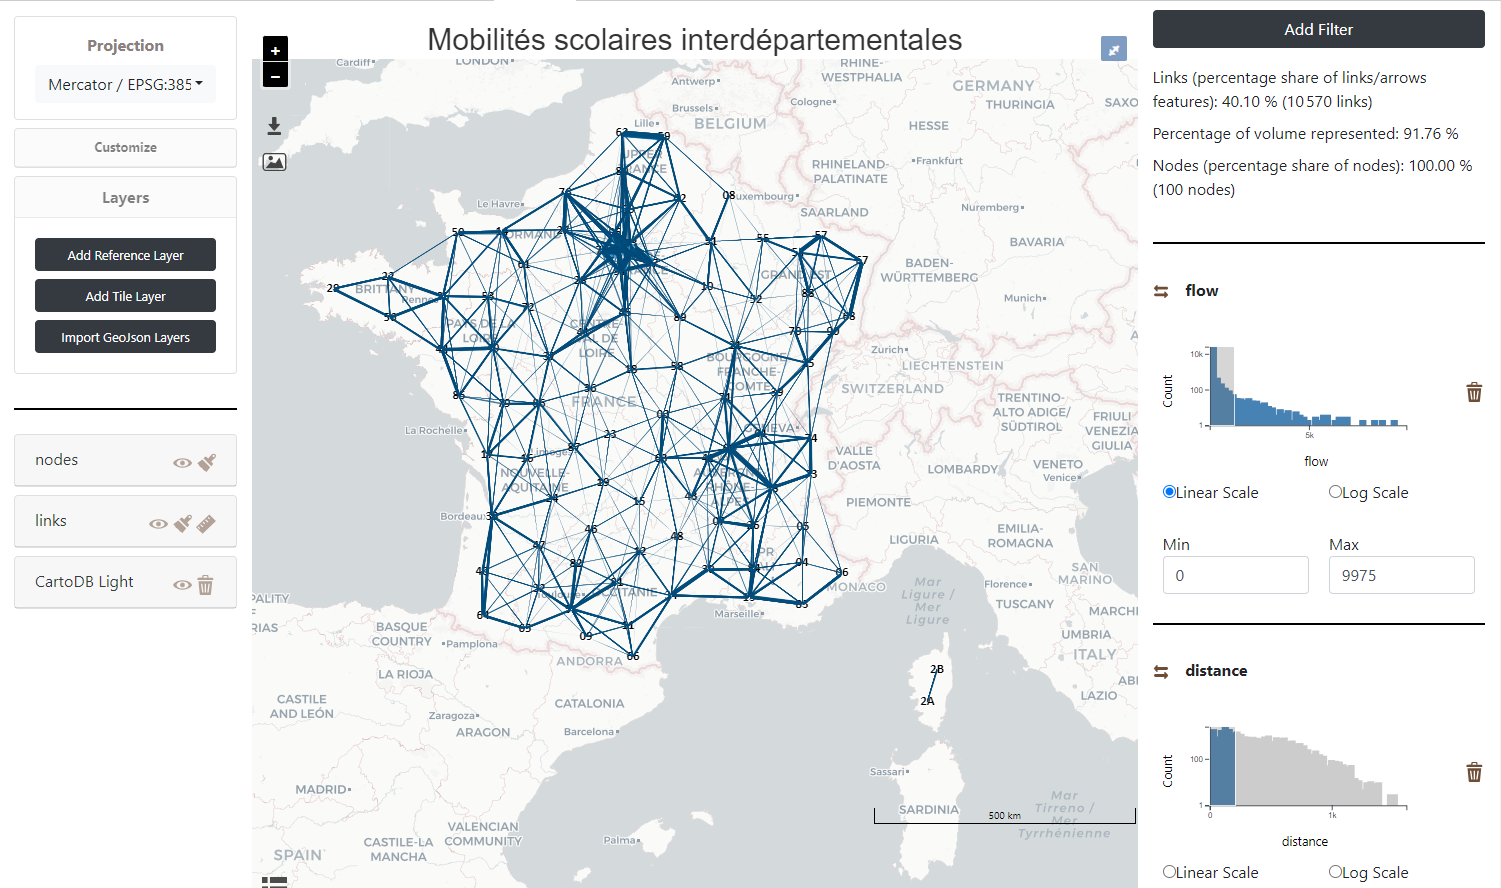
\includegraphics{images/panels_arabesque.png}

\section{The central panel}\label{the-central-panel}

The central part of Arabesque corresponds to the \textbf{map view}. It
results from the choice of the layers to be displayed (from the left
panel) and the filtering of the values of the links and nodes (from the
right panel).

This central panel also presents different buttons allowing the
implementation of primary actions.

\subsection{Primary actions with
butons}\label{primary-actions-with-butons}

The white page of Arabesque is decorated with blue action buttons.

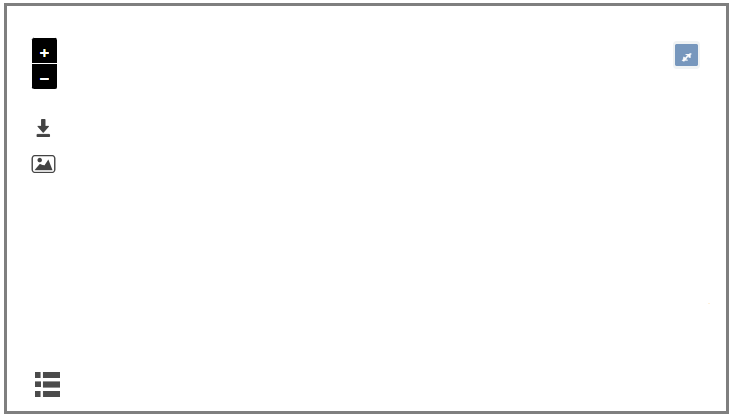
\includegraphics{images/central_panel_clear.png} \textbf{Details of the
different buttons}


\includegraphics{images/Buton_in_out.png} Successively zoom in/out - the
same way as with the mouse wheel.


\includegraphics{images/Buton_sauv.png} Save the project in .ZIP for
later use.


\includegraphics{images/Buton_export.png} Export the map in .PDF vector
format including legends in the bottom of the page.


\includegraphics{images/Buton_leg.png} Show/hide the legend.

\subsection{Primary legend}\label{primary-legend}

A legend is automatically generated for each map for nodes and links
plot.

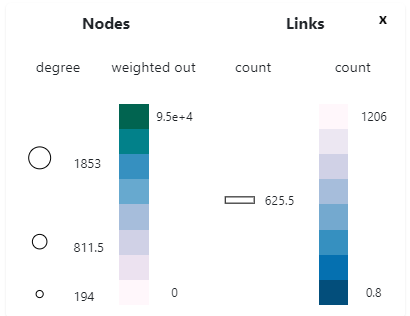
\includegraphics{images/center_legend.png}

The symbolization elements (size, color and opacity) of the nodes and
links are included in the legend. Here (for a default map), it is the
volume of flows and the degree of places that are represented.

\section{The geographic panel}\label{the-geographic-panel}

The left panel is to \textbf{design the map}:

\begin{itemize}
\item
  dealing with the map background as the geographical/geometrical
  layers: Arabesque reference layer, Tile Layer or your own geojson
  layers
\item
  customize the \emph{design}/style of the nodes and links features map.
\end{itemize}

The management of geographic information is composed of three
sub-sections:

\begin{figure}[H]

{\centering 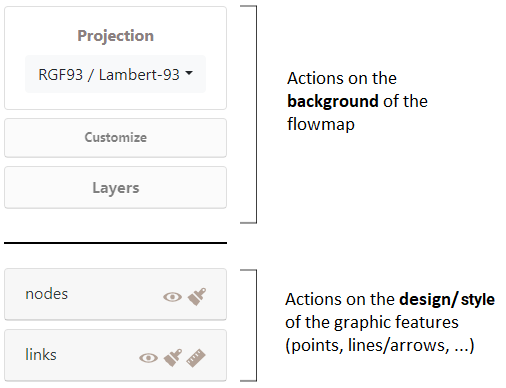
\includegraphics{images/geom_panel.png}

}

\caption{General geographic information management panel}

\end{figure}%

Actions on the \textbf{background of the map} are for changing
projections of the current map and/or to add other layers : remote or
personal one.

See \href{./Design-map-background.html}{Design map background} section.

Actions on the design/style is to set the parameters for the geometry of
the lines/arrows and their semiology

See \href{./Design-flowmap-signs.html}{Design flowmap signs} section.

\subsection{The geographic layer
manager}\label{the-geographic-layer-manager}

In practice, a map is composed by several layer such as the bounding
boxes, the graticules, the countries of land. All can be loaded in the
map design background section Layers.

They then appear in the layer manager sub-panel, one above the other as
shown below.

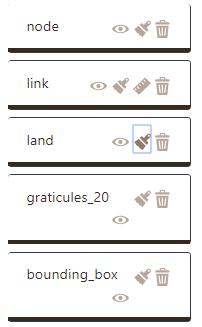
\includegraphics{images/Types_layers.png}

The present layers are all available on the map - but not necessarily
all of them are visible.

The layers on the view are positioned in an order that affects their
visibility. The top layer will be visible in the foreground.

\subsection{Layer rearrangement}\label{layer-rearrangement}

The drawing of the different layers and their objects can be finely
parameterized in \emph{Arabesque}, in order to take into account the
possible complexity of the information (density of the matrix) which
requires a particular management of the superimpositions and the
arrangements of the layers of links and nodes.

In the example below, the largest links are placed in the foregroundby
default, while the largest circles are not. After their rearrangement,
the largest links are background and their color intensity has been
changed (See Chapter \href{./Design-flowmap-signs.html}{Designing
flowmap signs}).

\emph{EXAMPLE:} rearrangement of nodes and links.

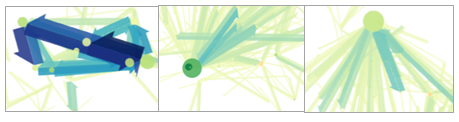
\includegraphics{images/Dispositions.png}

The position of the layers above and below (foreground/lowerground) can
be modified by a simple drag and drop.

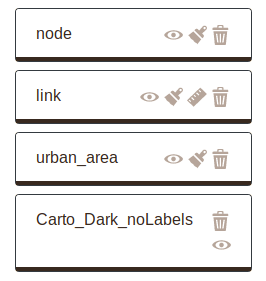
\includegraphics{images/Layout_dragdrop.png}

\begin{quote}
\textbf{\emph{Do it yourself !}}:

-- Click on the link layer and hold it down;

-- Drag/drop the link layer and place it in the foreground;

-- Release the layer;

-- Repeat the same operation with the node layer if necessary.
\end{quote}

After that, it can be seen that the layer of links has just been brought
to the forefront.

\section{The statistical panel}\label{the-statistical-panel}

The \textbf{right panel} is for playing with the flow data sets : the
nodes and/or links in order to \textbf{filter the map} with the Add
filter button.


\includegraphics{images/Add_filter.PNG}

The statistics panel describes also the share (as a percentage) of flow
information that is represented in the central view, before/after the
application of a filter.

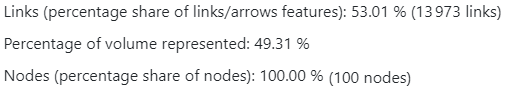
\includegraphics{images/Filter_statistics.png}

\begin{quote}
\textbf{\emph{Interpretation:}}

-- for links: 1.3973 links are depicted on the map, i.e.~53.01\% of the
total number of links, which corresponds to a density (or matrix fill
rate) of 53.01\%. These links represent 49.31\% of the total
interaction.

-- for nodes: 100\% of nodes are represented (here N=100 nodes)
\end{quote}

The filters applied are displayed in the second part of the panel,
depending on the type of data (continuous, categorical, etc.). See


\includegraphics{images/icon_links_filtering.png} Filter on a link
attribute


\includegraphics{images/icon_nodes_filtering.png} Filter on a node
attribute

See filtering flow data section.

\bookmarksetup{startatroot}

\chapter{Data importation}\label{data-importation}

Arabesque also allows you to import your own data sets via the home
page, in order to create a new map.

At least a link/flow origin-destination data file is required,
formatting with three colums. A node file is also required for the
geolocalisation of the origin and destination places.

In Arabesque 2, you have to declare or to import your nodes firstly.

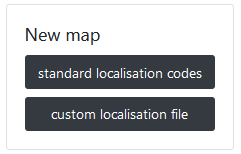
\includegraphics{images/Arabesque_homepage_newmap.png}

For this tutorial, we will use for example the historical trade flows
listed in the mobscol file. For more informations about this dataset see
in arabesque-examples.

\section{Nodes importation}\label{nodes-importation}

If your nodes are specific, see
\hyperref[custom-localisation-file]{Custom localisation file}, otherwise
you can use predefined locations with
\hyperref[standard-localisation-codes]{Standard localisation codes}.

\subsection{Standard localisation
codes}\label{standard-localisation-codes}

\begin{center}

\includegraphics{images/Nodes_import_standard.PNG}
\end{center}

Arabesque provides a list of codes identifying the most common spatial
units at different geographical scales, at global, at European or at a
national level.


\includegraphics{images/Preset.PNG}

At global level, for example, different grids are available (countries,
towns, ports, etc.).

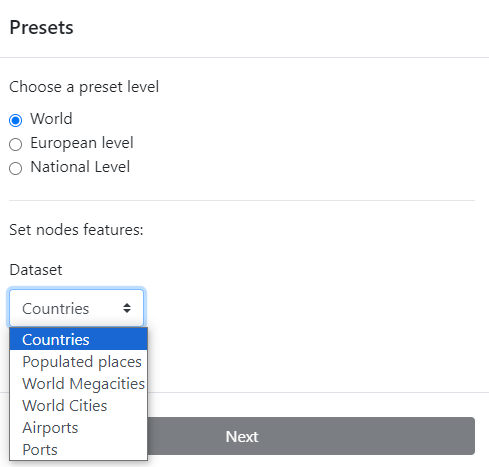
\includegraphics{images/Preset_world_countries.png}

The choice of the world country level, for example, then leads to the
identification of the type of identifier code: ISO2, ISO3, etc.

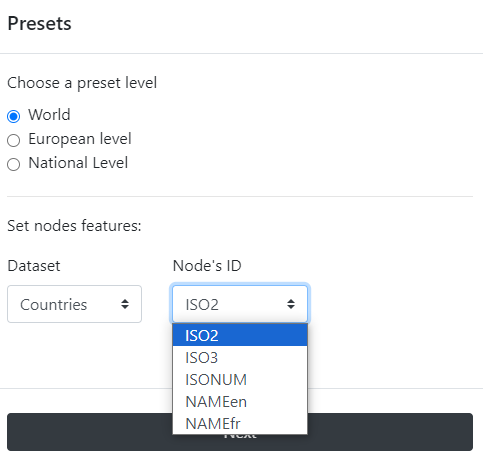
\includegraphics{images/Preset_world_countries_iso.png}

Once the type of identifier code has been selected (e.g.~ISO2), the link
file must be chosen.

\begin{center}
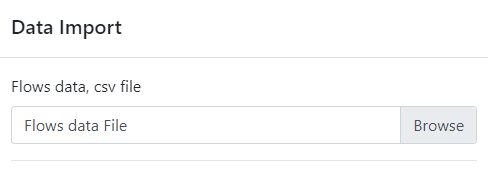
\includegraphics{images/Flow_import.PNG}
\end{center}

\subsection{Custom localisation file}\label{custom-localisation-file}

If you have custom nodes data associated with your ODs, you can load the
corresponding files by selecting the custom button.

\begin{center}

\includegraphics{images/Nodes_import_custom.PNG}
\end{center}

Then you have to browse to pick a .CSV or a GEOJSON file.

The .CSV file must be in long format, and have separator : , and decimal
: .

See example below.

\begin{quote}
Example: the SAGEO\_RIcardo\_nodes.CSV file
\end{quote}

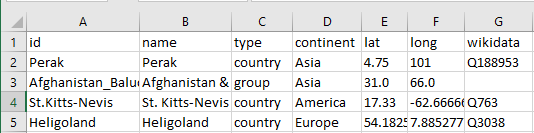
\includegraphics{images/Example_RICarto_nodes.PNG}

The most important here are the column `lat' (Y) and `long' (X) which
will be used to geolocate the origin and the destination places, then
the column `ID'

Once you have identified these three columns (ID, lat, long), you can
import the nodes.

\begin{center}
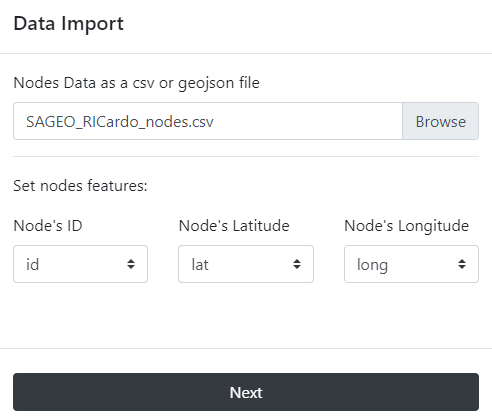
\includegraphics{images/Nodes_custom_import.PNG}
\end{center}

If you do not have a file for the geometry, you can use the codes
identifying the reference data (e.g.~INSEE codes of the French communes,
ISO codes of the countries), to automatically geolocate your nodes. See
Preset.

\section{Flow/links importation}\label{flowlinks-importation}

After loading the nodes files, you have to browse your directories to
upload your origin-destination matrix.

The flow/links file must be in \textbf{.CSV (separator : , and decimal :
.}) in \textbf{long format}.

It must contain at least 3 columns : the ID of the place of origin, the
ID of the place of destination locations and the flow values.

\subsection{Unique flow OD matrices}\label{unique-flow-od-matrices}

Unique OD matrices have a unique value for each pair of locations - this
makes them different from complex matrices {[}See
\hyperref[complex-od-matrices]{Complex OD matrices}{]}.

See example below.

\begin{quote}
Example: the Mobscol origin-destination .CSV file. Simple matrice with 3
columns.

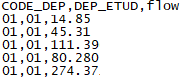
\includegraphics{images/Example_mobscol_ODsimple_CSV.PNG}
\end{quote}

The ID of the place of origin is ``CODE\_DEP''.

The ID of the place of destination is ``DEP\_ETUD''

The flow value is ``flow'' or is ``count''.

Once the origin and destination IDs have been identified, they need to
be declared in Arabesque for importing flows.

\begin{center}
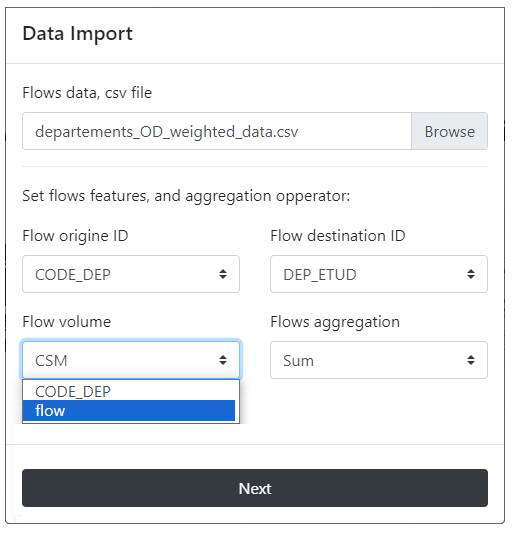
\includegraphics{images/Flowdata_import_simple.png}
\end{center}

If the matrix is complex (as in that example), you have to choose a
method for aggregating the links when importing. {[}See
\hyperref[complex-od-matrices]{Complex OD matrices}{]}

\subsection{Complex OD matrices}\label{complex-od-matrices}

The matrices concerned here are characterized by several attributes, for
categorical matrices (e.g.~flows that concern several social groups,
several goods transported) or for temporal matrices (e.g.~flows occur on
several dates).

If so, agregations procedures are suggested when importing the dataset
in \emph{Arabesque}. By default, the sum function is applied in the lack
of any other specifications. However, you can choose to apply an
average, minimum, maximum or median function calculated on all the
matrices or graphs provided.

It is also possible to choose a single date or to aggregate the data,
according to a given function, over a period or for categories.

\begin{quote}
Example: the Mobscol origin-destination. Complex matrice.

.CSV format

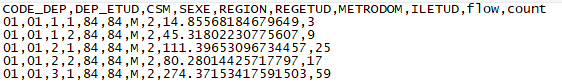
\includegraphics{images/Example_mobscol_OD_CSV.PNG}

.XLXS format.

\begin{center}
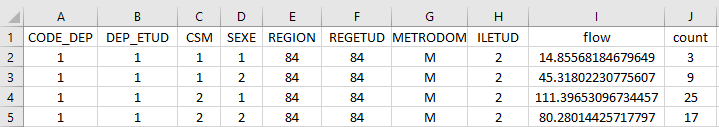
\includegraphics{images/Example_mobscol_OD.PNG}
\end{center}
\end{quote}

This OD matrix is available for different categories (i.e.~SEXE=``1'' or
SEXE=``2''), so you will need to choose a method for aggregating the
links when importing, hereby the sum function.

\begin{center}
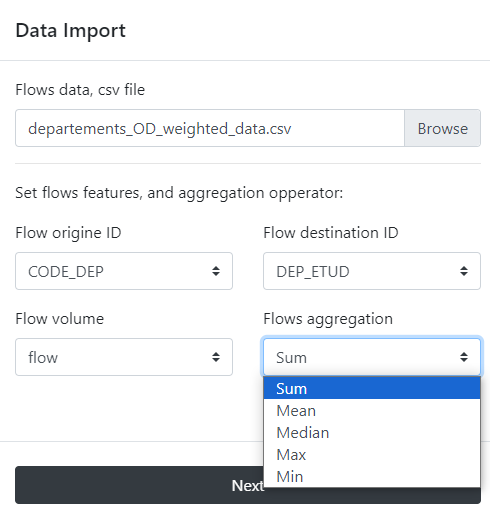
\includegraphics{images/Flowdata_import_aggregation.png}
\end{center}

This aggregation function is important because it defines the default
flowmap which will be proposed at the entry of \emph{Arabesque}: the
percent of links, nodes and interaction depicted, the intensity of the
colors and the opacity of the corresponding signs (see Data processing
chapter).

After aggregation, Arabesque will draws only one line (and not as many
lines for each attribute in the flow file).

\begin{tcolorbox}[enhanced jigsaw, rightrule=.15mm, bottomrule=.15mm, colback=white, breakable, opacityback=0, colframe=quarto-callout-note-color-frame, toprule=.15mm, leftrule=.75mm, arc=.35mm, left=2mm]
\begin{minipage}[t]{5.5mm}
\textcolor{quarto-callout-note-color}{\faInfo}
\end{minipage}%
\begin{minipage}[t]{\textwidth - 5.5mm}

\vspace{-3mm}\textbf{Note:}\vspace{3mm}

This aggregation does not interfere with the geo-visualization
possibilities that will remain available for all existing attributes.
The flow mapping according to one of these attributes can be performed
in the filtering section.

\end{minipage}%
\end{tcolorbox}

After loading the link and node files, Arabesque automatically performs
a join of the common attributes between the two files.

\section{Checking missing nodes/links
features}\label{checking-missing-nodeslinks-features}

Links that do not have an origin and/or destination ID are automatically
deleted. Nodes that don't have an ID code that allows them to be
geographically located are also not kept.

The list of links and nodes that may have been delete during the
importation procedure is displayed in a new window.

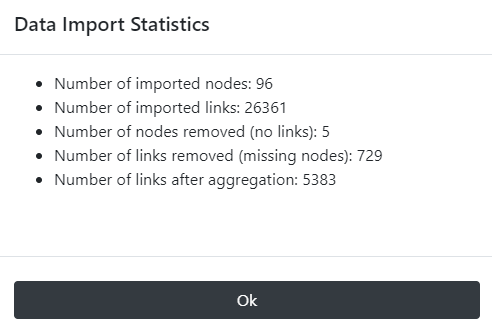
\includegraphics{images/import_suppr_entities.png}

This list is for quick reference only. You must copy and paste it (into
a text file, for example) if you want to keep the summary of the deleted
entities : here 5 nodes and 729 likns. Nodes have been deleted because
they are not related to other nodes.

After loading the link and node files, Arabesque automatically performs
a join of the common attributes between the two files and computes
indicator on botk links and nodes data.

\section{Import a previous workspace}\label{import-a-previous-workspace}

Import a previously workspace of flowmapping by loading a project file
in .zip format.

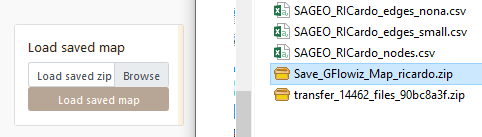
\includegraphics{images/import_zipfile.png}

\begin{tcolorbox}[enhanced jigsaw, rightrule=.15mm, bottomrule=.15mm, colback=white, breakable, opacityback=0, colframe=quarto-callout-warning-color-frame, toprule=.15mm, leftrule=.75mm, arc=.35mm, left=2mm]
\begin{minipage}[t]{5.5mm}
\textcolor{quarto-callout-warning-color}{\faExclamationTriangle}
\end{minipage}%
\begin{minipage}[t]{\textwidth - 5.5mm}

\vspace{-3mm}\textbf{.zip file}\vspace{3mm}

Do not modify this .zipfile, otherwise it will no longer work with
Arabesque, and you will not be able to load your workspace.

\end{minipage}%
\end{tcolorbox}

\bookmarksetup{startatroot}

\chapter{Data pre processing}\label{data-pre-processing}

After loading the data, the creation of a flow map with Arabesque can be
broken down into the following main steps.

\begin{tcolorbox}[enhanced jigsaw, rightrule=.15mm, bottomrule=.15mm, colback=white, breakable, opacityback=0, colframe=quarto-callout-tip-color-frame, toprule=.15mm, leftrule=.75mm, arc=.35mm, left=2mm]
\begin{minipage}[t]{5.5mm}
\textcolor{quarto-callout-tip-color}{\faLightbulb}
\end{minipage}%
\begin{minipage}[t]{\textwidth - 5.5mm}

\vspace{-3mm}\textbf{Flow mapping tips}\vspace{3mm}

\begin{enumerate}
\def\labelenumi{\arabic{enumi}.}
\tightlist
\item
  Importing flow data (links/nodes)
\item
  Processing flow data (automatic indicators calculation, \ldots)
\item
  Geographical data computing (layering, \ldots)
\item
  Statistical data computing (filtering, \ldots)
\item
  Designing links and arrows (geometry and semiology)
\item
  Designing nodes (semiology)
\item
  Map cosmetics (title, sources, \ldots)
\item
  Export
\end{enumerate}

\end{minipage}%
\end{tcolorbox}

The links and nodes datasets are automatically modified by creating new
columns when importing. Arabesque computes different key indicators and
a default flow map is suggested.

\section{Indicators on links}\label{indicators-on-links}

For the moment, only the euclidean distance between the origin and
destination entities is calculated.

\section{Indicators on nodes}\label{indicators-on-nodes}

A list of various simple and weighted indicators are calculated on the
nodes (with reference to the Social Network Analysis (SNA) theory are
proposed.

\textbf{balance} : difference between the number of in and out degrees.

\textbf{outdegree} : number of outgoing links from a places

\textbf{indegree} : number of ingoing links from a places

\textbf{weigthed Balance} : difference between the number of in and out
degrees weighted by the flow value (.ie. volume)

\textbf{weigthed degree} : difference between the number of ingoing and
outgoing links weigthed by the flow value (.ie. volume).

See below the additional indicators automatically calculated on the
nodes of the RIcardo data

See below the \textbf{Additional variables} that have been automatically
computed (ie the additional variable) on the nodes of the RIcardo data.

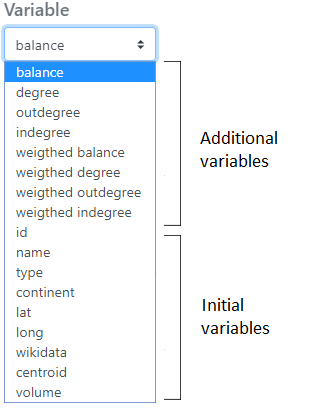
\includegraphics{images/import_indic.png}

These indicators can be downloaded in . csv format (see Export and Save
sections).

Loading links and nodes data into \emph{Arabesque} leads to the creation
of a default map, which is placed in the center of the interface.

\section{Suggested default flowmap}\label{suggested-default-flowmap}

Loading data in Arabesque leads to the creation of a default map to
avoid visualizing a ``spaghetti effect'' when entering the application ;
all the defined parameters can then be modified during the exploration.

By default, the links are represented in shades of blue and the nodes in
red. The map is presented in the WGS84 projection, according to the
lat/lon coordinates declared during the import.

Except in the case of loading a projected geometry as input, the map is
presented in WGS84.

Hereby is the Mobscol dataset default map in the central panel.

\textbf{For all default map, only a small percent ( around 10\%) of the
most important links (in value) are represented} and symbolized (see the
automatic legend) according to their intensity (the flow variable
entered at import).

The corresponding nodes are symbolized according to their degree
(automatically calculated variable during the import). Their ID codes
declared at the time of importation are also presented by default.

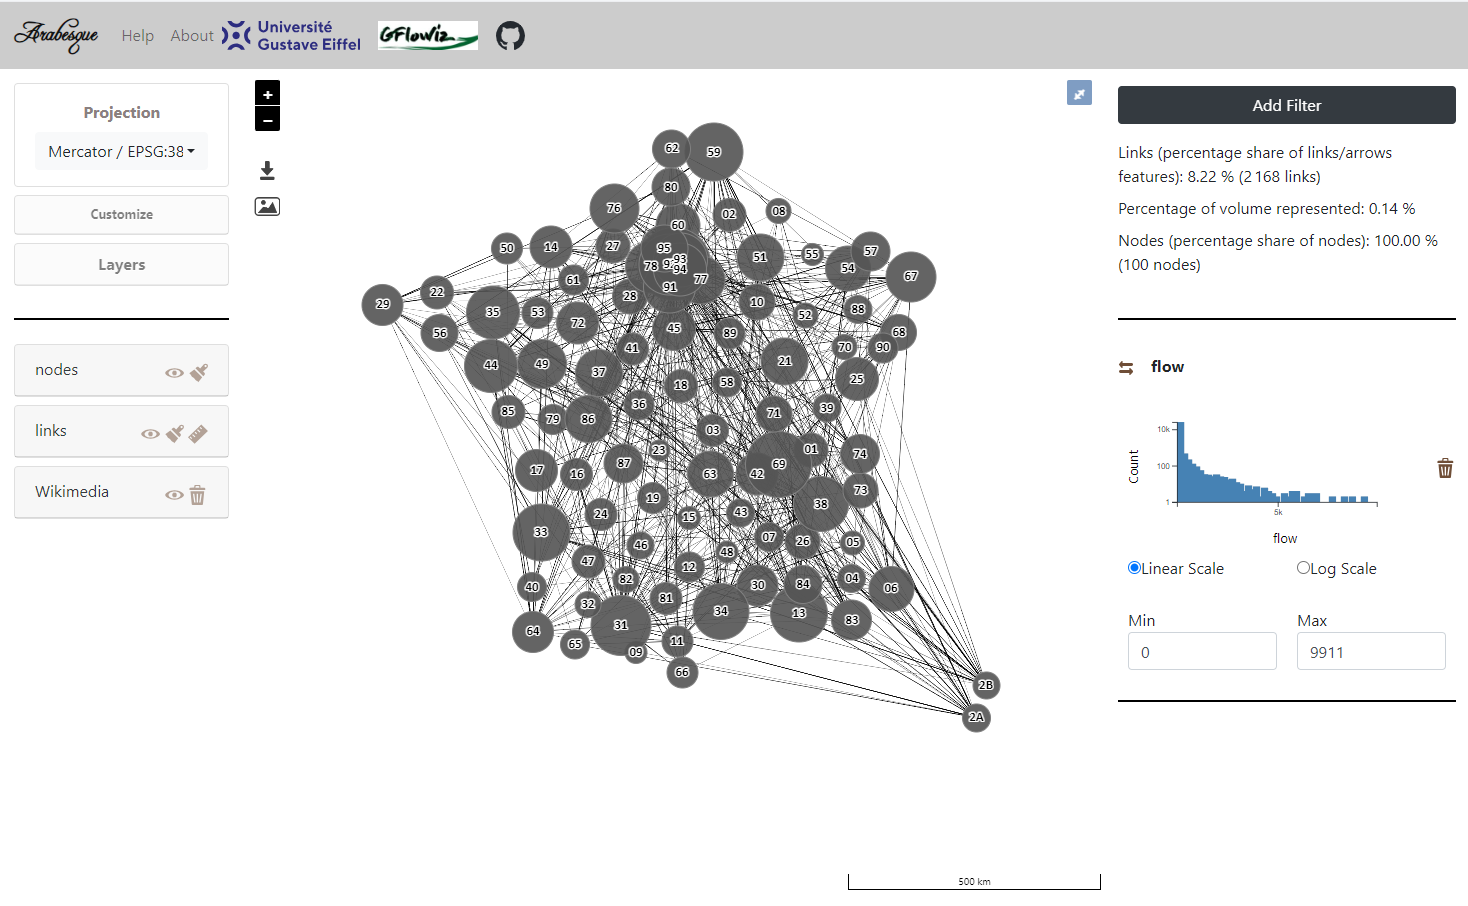
\includegraphics{images/default_flowmap-mobscol.png}

The right-hand panel shows :

- overall statistics on the proportion of flow information represented
on the map ;

- a flow value distribution diagram

All graphic and data filtering parameters can be modified using the left
(geography and semiology) and right (statistical filtering) panels.

\bookmarksetup{startatroot}

\chapter{Geographical data computing}\label{geographical-data-computing}

This chapter is about re projecting geographical layers, adding external
or personal layers as the flow map background, and their customization.

First you can project or reproject your layers.

\section{(re)Projecting layers}\label{reprojecting-layers}

The cartographic projection of the layers can be changed, by choosing
one of the proposed formulas in the projection menu.

\begin{center}
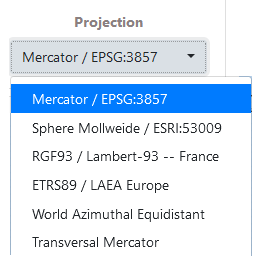
\includegraphics{images/Geo_projection.png}
\end{center}

\begin{quote}
Example: several projections applied on the RICardo world trade map
\end{quote}

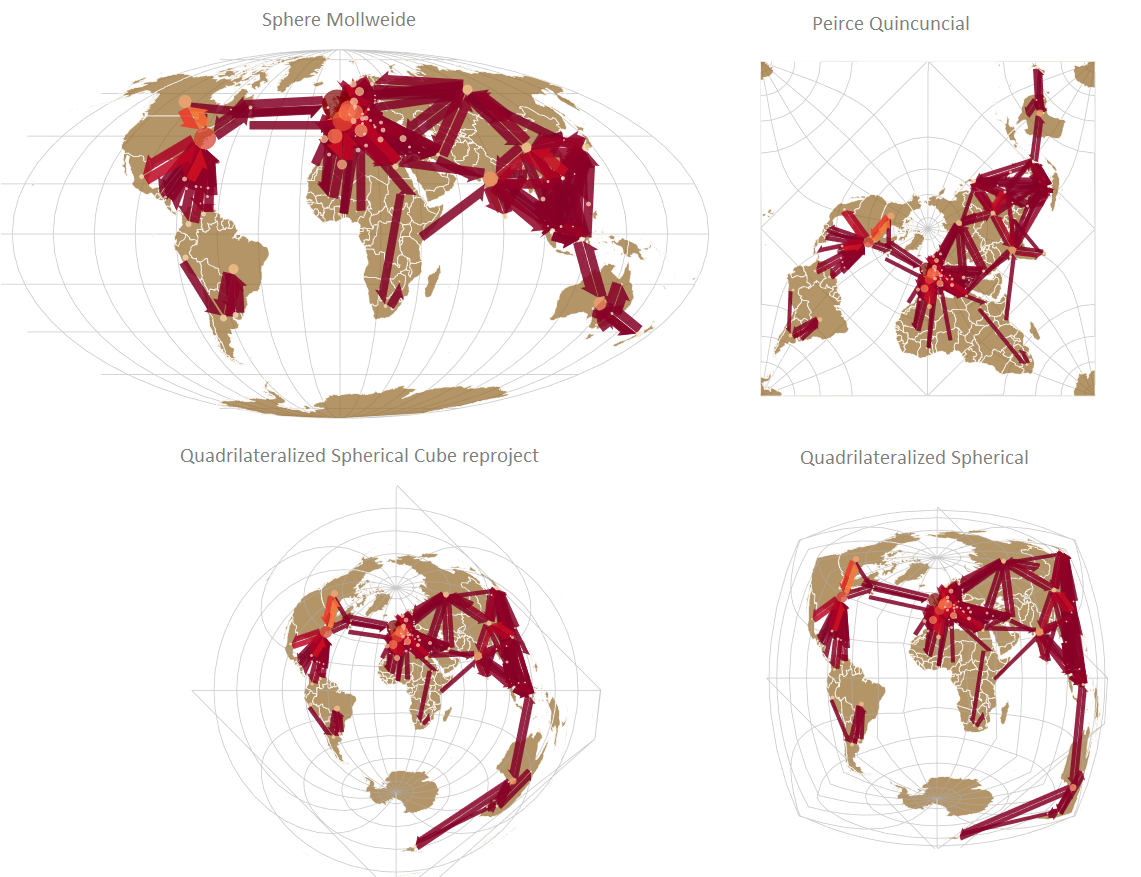
\includegraphics{images/RIcardo_reprojection.png}

\section{Geographical layers}\label{geographical-layers}

The management of the map background is related to the geographic
information. It can be accessed via the Layer button, and is composed of
three sub-sections.

\begin{center}
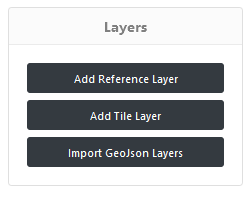
\includegraphics{images/Geo_layers.PNG}
\end{center}

\subsection{Add reference layer}\label{add-reference-layer}

Add reference layers consists in calling a remote geographic information
layer from Natural Earth data features, to contextualize the flowmap.

\begin{center}

\includegraphics{images/Add_reference_layer.PNG}
\end{center}

\begin{center}
\includegraphics{images/Geo_Add_reference_layer.png}
\end{center}

Selected reference layers are:

\begin{itemize}
\item
  geographical graticules are grids at 5, 10, 15, 20 and 30° intervals.
  Includes WGS84 bounding box.
  \href{https://www.naturalearthdata.com/downloads/50m-physical-vectors/50m-graticules/}{See
  details\ldots{}}

  \begin{quote}
  Example: Add graticule layer 20° interval
  \end{quote}

  \begin{center}
  \includegraphics{images/Add_reference_Layer_Graticule.png}
  \end{center}
\item
  world's countries divisions at spatial resolutions of 110 meters or 50
  meters, and the disputed areas.
  \href{https://www.naturalearthdata.com/downloads/10m-cultural-vectors/10m-admin-0-countries/}{See
  details\ldots{}}
\end{itemize}

\begin{quote}
Example: countries
\end{quote}

\begin{center}
\includegraphics{images/Add_reference_Layer_Country.png}
\end{center}

\begin{itemize}
\item
  world urban areas (of dense human habitations) coverage derived from
  MODIS satellite, at spatial resolutions of 50 meters or 10 meters.
  \href{https://www.naturalearthdata.com/downloads/50m-cultural-vectors/50m-urban-areas/}{See
  details\ldots{}}
\item
  world landscape based on lands including major islands.
  \href{https://www.naturalearthdata.com/downloads/10m-physical-vectors/10m-land/}{See
  details\ldots{}}
\end{itemize}

For all these layers, their fill and stroke can be defined by picking
colors, then click on Add layer button.

\subsection{Add tile layer}\label{add-tile-layer}

The Base type of tiles layers come from Open Street Map (OSM)
\href{https://wiki.openstreetmap.org/wiki/Tile_servers}{tile server},
CARTO DB and
\href{https://enterprise.arcgis.com/fr/server/latest/publish-services/linux/vector-tile-services.htm}{ESRI
tile server}.

\begin{center}
\includegraphics{images/Add_tyle_layer.PNG}
\end{center}

\includegraphics{images/Geo_Add_tile_layer.png}

\subsection{Add Geojson layer}\label{add-geojson-layer}

Import Geojson is to load a personal vector layer.

\begin{center}
\includegraphics{images/Geo_Add_geojson.png}
\end{center}

\section{Layer management}\label{layer-management}

Displaying geographic information layers adds layers in the Layer
management section. Depending on their position, the added layers
(hereby Land 110m and graticules 20) can hide the initial node and link
layers, with the most recently added layers in the foreground.

\includegraphics{images/Dispositions_all.png}

\subsection{Changing the layer layout}\label{changing-the-layer-layout}

To make the new layer visible in a correct order, you need to change the
layout of the different layers, by modifying their order by drag \&
drop.

\begin{itemize}
\item
  Click and hold on the link layer;
\item
  Drag and drop the link layer to the foreground;
\item
  Release the layer;
\item
  Repeat the same operation with the node layer if necessary.

  \includegraphics{images/Dispositions_all_change.png}

  \subsection{Manage the visibility of a
  layer}\label{manage-the-visibility-of-a-layer}
\item
  Differents icons are useful to manage the layers' appearance.

  \includegraphics{images/buton_hide.png} Hide a layer

  \includegraphics{images/Buton_show.png} Show a layer (make it visible)

  \includegraphics{images/Buton_action_delete.png} Delete a layer
\item
  Icons for modifying the design of a layer
\end{itemize}

\includegraphics{images/Buton_action_semio.png} Semiology parameters of
flow features (nodes and links) : color, size, text, opacity.

\includegraphics{images/Buton_action_geom.png} Geometry parameters for
changing links/arrows shape only. This is not available for nodes). It
is possible to change their orientation, the type of link (curve,
triange, \ldots) and arrow head parameters.

\bookmarksetup{startatroot}

\chapter{Designing the links/arrows}\label{designing-the-linksarrows}

This chapter concerns the drawing of the links features : their
geometry/shape and their semiology.

Sign parameters are set on the left panel - in the layer management
section ie. the lower part, which displays at least two geographical
layers : one on links and one on nodes.

\includegraphics{images/geom_panel_flowsigns.png}

\begin{tcolorbox}[enhanced jigsaw, coltitle=black, opacitybacktitle=0.6, title=\textcolor{quarto-callout-note-color}{\faInfo}\hspace{0.5em}{Note:}, bottomtitle=1mm, colframe=quarto-callout-note-color-frame, leftrule=.75mm, arc=.35mm, left=2mm, colbacktitle=quarto-callout-note-color!10!white, toptitle=1mm, bottomrule=.15mm, colback=white, breakable, opacityback=0, rightrule=.15mm, toprule=.15mm, titlerule=0mm]

Other geographic information layers (tiles, \ldots) can also be
displayed in this section.

\end{tcolorbox}

\section{Designing the links}\label{designing-the-links}

the design of the links can be modified in two ways: their semiology and
their geometry by using the following icons:

\includegraphics{./images/Icon_links_geom.png} Modify the style of the
links

\section{Links's semiology}\label{linkss-semiology}

\includegraphics{images/Buton_action_semio.png} Three semiological
parameters are available for designing the links : their color, their
size and their opacity.

\includegraphics{./images/Links_change_style.png}

\section{Links' geometry parameters}\label{links-geometry-parameters}

Geometry parameter is to change arrow shape

\includegraphics{images/Buton_action_geom.png} Three geometrical
parameters are available for designing the links : their shape, their
type, their arrow head and their width

\includegraphics{images/Design_links_arrows.png}

\subsection{Links' orientation}\label{links-orientation}

The link can be oriented in the form of an arrow or not (remain as a
simple line).

\includegraphics{images/geom_add_links_geometry1.png}

Oriented geometry takes into account the direction of the \textbf{flow}
to define the \textbf{graphic form} of the sign.

\begin{tcolorbox}[enhanced jigsaw, rightrule=.15mm, bottomrule=.15mm, colback=white, breakable, opacityback=0, colframe=quarto-callout-note-color-frame, toprule=.15mm, leftrule=.75mm, arc=.35mm, left=2mm]
\begin{minipage}[t]{5.5mm}
\textcolor{quarto-callout-note-color}{\faInfo}
\end{minipage}%
\begin{minipage}[t]{\textwidth - 5.5mm}

\vspace{-3mm}\textbf{Note about to the orientation}\vspace{3mm}

The link's orientation is related to the declared from-to parameter
adjusted when the links were imported. See Data importation chapter.

\end{minipage}%
\end{tcolorbox}

\subsection{\texorpdfstring{\textbf{Link's
types}}{Link's types}}\label{links-types}

Five forms of flow lines are available.

\begin{itemize}
\item
  \textbf{straight} ;
\item
  \textbf{straight no hook} ;
\item
  \textbf{triangle} ;
\item
  (line) \textbf{curve}
\item
  \textbf{Triangle curve}.
\end{itemize}

\includegraphics{images/Links_geom.png}

\begin{itemize}
\item
  \textbf{Straight} (as euclidian distance symbolisation): The link is
  straight and oriented, with a half arrowhead.
\item
  \textbf{Straight no hook}: The link is straight and oriented, it has a
  point without hook.
\item
  \textbf{Triangle}: The link is straight and takes the shape of a
  triangle.
\item
  \textbf{Curve} : The link is curved and oriented, its curvature is
  configurable in the Arrow head section if selected.
\item
  \textbf{Triangle curve}: The link is curved and takes the shape of a
  drop of water, its curvature is configurable in the Arrow head section
  if selected.
\item
  \textbf{Non oriented}: The link is straight, valuate or not, it has no
  direction.
\end{itemize}

The arrow geometry - which corresponds to the visual shape variable -
can be rectilinear or curvilinear.

\subsection{Design of linear arrows}\label{design-of-linear-arrows}

The \textbf{straight} and \textbf{straight no hook} type of line
(oriented as arrows or not) is for rectilinear flow features.

Only the \textbf{arrow head} can be set if required.

\includegraphics{images/geom_add_links_straight.png}

\begin{itemize}
\item
  \textbf{Arrow head-Height} (curve): The value of the height of the
  head is the percentage of the map distance of the link (distance
  between the origin and the destination) used to define the maximum
  (map) width of the link
\item
  \textbf{Arrow head-Width} being itself a function of the value of the
  flow, but it can be set as constant here.
\end{itemize}

\subsection{Design curved lines/arrows}\label{design-curved-linesarrows}

The curvature of the line is generated according to the Chaikin
algorithm which allows to parameterize its height and its base, with
respect to the body of the link.

\begin{center}
\includegraphics{images/Add_links_curve_arrow.png}
\end{center}

\begin{itemize}
\item
  \textbf{Height curve}: the ({[}0,5{]} is identified as a distance from
  the origin node of the link. Here, the point is approximately in the
  middle of the curve.
\item
  \textbf{Center Curve:} the value of ({[}0,5{]}) is that of the center
  of the curve for a pseudo 3D rendering.
\end{itemize}

\bookmarksetup{startatroot}

\chapter{Designing the nodes of the
flowmap}\label{designing-the-nodes-of-the-flowmap}

This chapter concerns the drawing of the nodes, especially the
configuration of their semiology.

\begin{center}
\includegraphics{images/geom_panel_nodessigns.png}
\end{center}

\begin{tcolorbox}[enhanced jigsaw, rightrule=.15mm, bottomrule=.15mm, colback=white, breakable, opacityback=0, colframe=quarto-callout-note-color-frame, toprule=.15mm, leftrule=.75mm, arc=.35mm, left=2mm]
\begin{minipage}[t]{5.5mm}
\textcolor{quarto-callout-note-color}{\faInfo}
\end{minipage}%
\begin{minipage}[t]{\textwidth - 5.5mm}

\vspace{-3mm}\textbf{Note}\vspace{3mm}

Note: other geographic information layers (tiles, \ldots) can also be
displayed in this section.

\end{minipage}%
\end{tcolorbox}

\section{Nodes semiology}\label{nodes-semiology}

\includegraphics{images/Buton_action_semio.png} Three semiological
parameters are available for designing the links : their color, their
size their topononym or label and their opacity.

Hereby the general window for changing the semiology and the style of
the nodes, regarding three parameters : their color, their size and
their toponym (text).

\begin{center}
\includegraphics{images/Nodes_semio.PNG}
\end{center}

\section{\texorpdfstring{\textbf{Nodes'
color}}{Nodes' color}}\label{nodes-color}

The colour of a node can be set according to three criteria: a setting
mode, a variable and the type of the variable.

\subsection{Setting modes of the
color}\label{setting-modes-of-the-color}

\begin{itemize}
\tightlist
\item
  \textbf{Constant mode} means that the color of the nodes is fixed and
  identical for all nodes.
\end{itemize}

\includegraphics{images/Nodes_color_constant.png}

\begin{itemize}
\tightlist
\item
  \textbf{Conditional mode} means that the color of the nodes will vary
  according to the character value (of a variable)
\end{itemize}

\begin{center}
\includegraphics{images/Nodes_color_conditionnal.PNG}
\end{center}

The reference for the color schemes is Cynthia Brewer palette for
Diverging, Multi Hue and Single Hue. See:
\href{https://colorbrewer2.org/\#type=sequential&scheme=BuGn&n=3}{Color
Brewer advices for maps}. An Extra Palette is also proposed in
Arabesque.

\subsection{Colour variation as a function of a
variable}\label{colour-variation-as-a-function-of-a-variable}

The color of the nodes can be set according to one of the variables
(initial or calculated by Arabesque) that are available in the dataset.

\includegraphics{images/geom_add_nodes_1_color_variable.png}

\subsection{Colour variation as a function of the type of a
variable}\label{colour-variation-as-a-function-of-the-type-of-a-variable}

\begin{tcolorbox}[enhanced jigsaw, rightrule=.15mm, bottomrule=.15mm, colback=white, breakable, opacityback=0, colframe=quarto-callout-caution-color-frame, toprule=.15mm, leftrule=.75mm, arc=.35mm, left=2mm]
\begin{minipage}[t]{5.5mm}
\textcolor{quarto-callout-caution-color}{\faFire}
\end{minipage}%
\begin{minipage}[t]{\textwidth - 5.5mm}

\vspace{-3mm}\textbf{Caution}\vspace{3mm}

The type of color range (Diverging/Multi Hue/Single Hue/Extra Palette)
will have to be realized according to the type of the variable to
represent (quantitative/qualitative, discrete/continuous,
stock/ratio/scale, \ldots).

\end{minipage}%
\end{tcolorbox}

\includegraphics{images/geom_add_nodes_1_color_variable2.png}

The progression (up/down) of the \textbf{color range} depends on that of
the \textbf{value range}: it can be direct or inverse. The checked box
means an inverse progression: a light color is applied to a strong
value.

\includegraphics{images/geom_add_nodes_1_color_variable3.png}

\section{\texorpdfstring{\textbf{Node's
size}}{Node's size}}\label{nodes-size}

The size of the nodes can be fixed and the weight defined.

\includegraphics{images/geom_add_nodes_2_size.png}

\subsection{Nodes' size weighted by a
variable}\label{nodes-size-weighted-by-a-variable}

The size of the nodes can be \textbf{weighted by a variable} according
to one of the initial or additional \textbf{variables} available in the
dataset (hereby the balance).

\includegraphics{images/geom_add_nodes_2_size_variable.png}

Three functions to set the size of the node according to the
corresponding value are proposed: linear, square, square root and
logarithmic.s

\includegraphics{images/geom_add_nodes_2_size_fct.png}

\subsection{Nodes' size ratio}\label{nodes-size-ratio}

The \textbf{ratio} representing the max width in pixel of the graphic
features can be defined - according to the map bounding box, to obtain
an image with balanced features (neither too small nor too big).

\includegraphics{images/geom_add_nodes_2_size_ratio.png}

\section{\texorpdfstring{\textbf{Node's label
(text)}}{Node's label (text)}}\label{nodes-label-text}

Textual elements can also be added near the nodes.

\includegraphics{images/geom_add_nodes_3_texte.png}

The text can be defined according to one of the variable available in
the nodes' dataset, here the name, the type, etc..

The opacity of the text shade (currently set to black) can be set to a
given value (here 0.91).

\includegraphics{images/geom_add_nodes_3_texte_fixe.png}

The opacity of the text shade (currently set to black) can be varied
according to an indicator present in the dataset, that is to say : the
nodes' original variables and the precalculated ones (degree, \ldots).

\includegraphics{images/geom_add_nodes_3_texte_variable.png}

\section{The nodes' geometric
parameters}\label{the-nodes-geometric-parameters}

Not implemented yet. Upcoming projects.

\bookmarksetup{startatroot}

\chapter{Filtering flowdata}\label{filtering-flowdata}

This chapter concerns the filtering procedures for flowdata in order to
reduce the graphic complexity of the flow map - the so-called
\emph{spaghetti effect}.

Filtering procedures are also important to select useful information:
links and/or nodes to obtain an interesting flowmap.

Without filtering, the flowmap patterns reveals a
\emph{spaghetti-effect}. See example

\emph{EXAMPLE:} RICardo international trade flows like a dish of
spaghetti.

\begin{center}
\includegraphics{images/RICardo_spaghetti.png}
\end{center}

The selected information shown is described in percent on the bottom of
the right panel. Here, all the information is represented :100\% of the
links,100\% of the nodes and 100\% of the total information).

Filtering can be performed in \emph{Arabesque} on all variables
describing the nodes and/or links.

\section{Available filtering
procedures}\label{available-filtering-procedures}

\subsection{Filtering possibilities}\label{filtering-possibilities}

Filtering is available on numerical, temporal and categorical variables.

\subsubsection{Numerical variables}\label{numerical-variables}

Numerical filtering applies to quantitative (absolute, continuous or
pseudo-continuous) dat is done either visually with a brush on an
interactive histogram or bar chart. It is also possible to indicate a
threshold.

\subsubsection{Temporal variables}\label{temporal-variables}

The filtering possibilities of the temporal matrices are currently only
available for links. They concern the choice of a date or a period, in a
numerical or graphical form (slider). Three date formats are available
(string, hours, timestamp).

\subsubsection{Categorical variables}\label{categorical-variables}

Categorical filtering is applied to nominal qualitative data available
in node and/or link datasets. Three possibilities are offered,
graphically and numerically:

-- \textbf{Selection of multiple variables}: the user chooses one or
more of the available categorical variables (e.g., prefectures and
sub-prefectures if a variable specifying the administrative profile of
French cities is available) or the type of links (e.g., import or export
for trade data);

-- \textbf{Selection of a single variable}: the user chooses a single
variable (for the nodes: for example, the flows from and to France for
mobility data; the import type flows for trade data);

-- \textbf{Selection by deletion of a single variable}: the user chooses
one or more variables relating to the nodes and links to be deleted. If
the deletion selection concerns nodes, all the corresponding links (for
example, the Ile-de-France region for an analysis at the national level)
are deleted.

\subsection{Implementing filtering}\label{implementing-filtering}

The \emph{Arabesque} filtering possibilities depend on the type of
variable/procedure of filtering, as well as the corresponding graph for
visual implementation.

Three main possibilities are proposed

-- (1) visual filtering using modular* \textbf{selection area (brush)}
applied on an histogram or an bar chart (see above) ;

-- (2) \textbf{numerical thresholding} by indicating a threshold ;

\includegraphics{images/schema_histogram.png}

\includegraphics{images/schema_BarChart.png}

-- (3) visual filtering \textbf{using a slider} (hereby, on links)

\includegraphics{images/schema_Slider_temp.png}

\section{Filtering by links}\label{filtering-by-links}

\includegraphics{images/icon_links_filtering.png} Icon indicating the
existence of a filtering possibility applied on the links.

\subsection{Add filter}\label{add-filter}

\includegraphics{images/Add_filter.PNG}

First, it is to click on Add filter on the bottom of the right panel,
then on Link in the opened window.

\includegraphics{images/Add_filter_links1.png}

The most common filtering consists in thresholding on the flow values
(the volume variable declared when importing the data)

\includegraphics{images/Add_filter_links_volume.png}

For links, the possibility of filtering according to the distance
traveled is also proposed.

It is possible to choose the variable - or declare/type its format in
order to draw an histogram for example.

\subsection{Choose the format of the variable to be
filtered}\label{choose-the-format-of-the-variable-to-be-filtered}

You must declare the type of data so that the corresponding graph can be
displayed to allow visual thresholding.

\includegraphics{images/Add_filter_links_volume_continuous.png}

\textbf{Categorial} is for qualitative categorical variables

\textbf{Continuous} is for filtering quantitative variable with the
slider on a measure or on an interval of values.

\textbf{Discrete} is for selecting one or more modality/measure relating
to links (and the corresponding nodes, and reversly) from be flowmap.

\textbf{Categorical} is for filtering on a single/several modality of a
qualitative variable

Above, the volume is declare as numeral for plotting the resulting map
with RICardo data set:

\includegraphics{images/Add_links_filter_volume_histogramme.png}

\begin{center}
\includegraphics{images/RICardo_filter_links_continuous.png}
\end{center}

The selected information shown is described in percent on the bottom of
the panel. Here only 2,6\% of the links and 15\% of the nodes represents
56\% of the total volume of trade flows.

The minimum and maximum values are automatically shown on the histogram.
It is possible to change these values by brushing on the histogram.

\subsection{Multi variables filtering}\label{multi-variables-filtering}

Several filter can be applied on links. Hereby, we add a second filter
on the distance variable.

\includegraphics{images/Add_filter_links_dist.png}

The two filter will then be available in the right panel (hereby, volume
and distance)

\includegraphics{images/Add_links_filter_vol_distance.png}

Only flows that have traveled less than 4900 km are depicted.

\subsection{Local filter of links: by origin or
destination}\label{local-filter-of-links-by-origin-or-destination}

It is also possible to filter the links by origin or by destination.

\includegraphics{images/Add_links_filter_origin.png}

Then, it is a matter of specifying a type, here categorical, to display
the flows issued from a country.

\includegraphics{images/Add_filter_links_origin_categorial.png}

You must then choose the country in the list or enter the name of the
selected one.

\begin{center}
\includegraphics{images/Add_filter_node_category_select.png}
\end{center}

Here we entered France.

\begin{center}
\includegraphics{images/Add_filter_links_origin_categorial_SelectFrance.png}
\end{center}

In order to display all flows from France, the (possible) other active
filters have been set to zero.

\includegraphics{images/Add_links_filter_origin_France.png}

\emph{NOTE}: in order to be able to see all the flows from one place of
origin (or destination), it is necessary to set the previous filters to
zero (but it is not necessary to delete them).

\subsection{Filter by a categorical
variable}\label{filter-by-a-categorical-variable}

It is possible to select several categorical variables (ie several
countries of origin).

\includegraphics{images/Add_filter_links_category.png}

\subsection{Filter by a temporal
variable}\label{filter-by-a-temporal-variable}

The filtering of temporal data considers different field formats: date,
hours and time stamp.

\includegraphics{images/Add_filter_links_temporal.png}

\subsection{Filter by a Remove}\label{filter-by-a-remove}

\section{Filtering by nodes}\label{filtering-by-nodes}

First, it is to click on Add filter, then on Node.

\includegraphics{images/icon_nodes_filtering.png} Icon indicating the
existence of a filtering possibility applied on the nodes.

\includegraphics{images/Add_filter_nodes1.png}

\bookmarksetup{startatroot}

\chapter{Flowmap cosmetics}\label{flowmap-cosmetics}

One of the new features of version 2 of Arabesque is this chapter
related to the customization of the map before exporting it.

You can enter a title, the author's name and the sources.

\begin{center}
\includegraphics{images/flowmap-customization.PNG}
\end{center}

You can enter a \textbf{title}, which will be placed at the top centre
of the map.

The \textbf{author's name} and \textbf{the sources} will be placed at
the bottom right of the map.

Other map editing functions will be added progressively.

\begin{tcolorbox}[enhanced jigsaw, rightrule=.15mm, bottomrule=.15mm, colback=white, breakable, opacityback=0, colframe=quarto-callout-note-color-frame, toprule=.15mm, leftrule=.75mm, arc=.35mm, left=2mm]
\begin{minipage}[t]{5.5mm}
\textcolor{quarto-callout-note-color}{\faInfo}
\end{minipage}%
\begin{minipage}[t]{\textwidth - 5.5mm}

\vspace{-3mm}\textbf{Note}\vspace{3mm}

When exporting the flow map, the name will also be the name of the
export file.

\end{minipage}%
\end{tcolorbox}

\bookmarksetup{startatroot}

\chapter*{References}\label{references}
\addcontentsline{toc}{chapter}{References}

\markboth{References}{References}

\section*{References quoted in the
documentation}\label{references-quoted-in-the-documentation}
\addcontentsline{toc}{section}{References quoted in the documentation}

\markright{References quoted in the documentation}

-- Equipe gflowiz (2019),
\href{https://github.com/gflowiz/sageo-ricardo}{Arabesque quick tutorial
v.0} for SAGEO 2019 - french version. Licence : CC-BY-SA 3.0-FR.

-- Mac Eachren A., (2005), \emph{How Maps Work, Representation,
Visualization, and Design}, New-York, The Guildford Press.

-- Girard P. et Dedinger B. (2020), Pourquoi et comment géolocaliser le
commerce mondial des XIXe-miXXe siècles ? : Retour d'expérience sur
l'usage de wikidata comme gazetteer historique et de l'application de
cartographie de flux Arabesque, Humanistica, Medialab Sciences-Po. et
Centre d'histoire de Sciences-Po.
\href{http://medialab.github.io/publications/geolocaliserRICardo@humanistica2020/}{Accéder}

\section*{\texorpdfstring{\textbf{Academic references on
Arabesque}}{Academic references on Arabesque}}\label{academic-references-on-arabesque}
\addcontentsline{toc}{section}{\textbf{Academic references on
Arabesque}}

\markright{\textbf{Academic references on Arabesque}}

(in descending chronological order, then by first author)

Bahoken F. (2023), \emph{Arabesque. La boîte à outils de cartographie et
de géovisualisation de données}, Journée d'études : regards croisés de
chercheurs, Jan 2023, Rennes, France. 53p.
\href{https://hal.science/hal-03948332}{〈hal-03948332〉}

Côme E., Bahoken F., Jégou L.( 2021), \emph{Arabesque : Explorer et
visualiser facilement vos flux géo-localisés sur le web}, Conférence,
Toulouse DataViz TDV2021, Apr 2021, Toulouse, France. 27p.
\href{https://hal.science/hal-03206235}{〈hal-03206235〉}

Roelandt N., Bahoken F., Le Campion G., Jégou L., Maisonobe M., et
al.~(2021), One Arabesque in the small world of OD webmaps. \emph{ISPRS
International Archives of the Photogrammetry, Remote Sensing and Spatial
Information Sciences}, 2021, 46, pp.147-154.
\href{https://dx.doi.org/10.5194/isprs-archives-xlvi-4-w2-2021-147-2021}{〈10.5194/isprs-archives-xlvi-4-w2-2021-147-2021〉}.
\href{https://hal.science/hal-03540581}{〈hal-03540581〉}

Bahoken F., Côme E., Jégou L. (2021) Arabesque, une application
d'exploration et de visualisation de flux dans le geoweb, Conférence
internationale \emph{Tous (im)mobiles, tous cartographes ? Cartomob},
Université Gustave Eiffel, Jun 2021, Toulouse, France.
\url{https://hal.science/hal-04411623}

Bahoken F., Le Campion G., Maisonobe M., Jégou L., Côme É. (2020), «
Typologie d'un geoweb des flux et réseaux / Typology of a flow and
network geoweb »\emph{, Géomatica Journal:} URL :
\url{https://cdnsciencepub.com/doi/abs/10.1139/geomat-2020-0007} ; DOI :
10.1139/geomat-2020-0007.

Côme E., Bapaume T., Jégou L., Bahoken F., Maisonobe M., Roelandt N., Le
Campion G. (2019), \emph{Arabesque}, application d'exploration et de
géovisualisation de données de flux et de réseaux, Conférence
internationale Spatial Analysis and Geomatics,
\href{https://sageo2019.irstea.fr/actes/}{Actes\_sageo2019} pp.~265-264.
\href{https://hal.science/hal-02299349}{〈hal-02299349〉}

Bahoken F., Le Campion G., Jégou L., Maisonobe M., Côme E. (2019),
\emph{Panorama d'un geoweb des flux et des réseaux} :
\href{https://sageo2019.irstea.fr/actes/}{Actes\_sageo2019},
pp.~218-231.

Equipe gflowiz (2019),
\href{https://github.com/gflowiz/sageo-ricardo}{Arabesque quick tutorial
v.0} for SAGEO 2019 - french version. Licence : CC-BY-SA 3.0-FR.

Mac Eachren A., (2005), \emph{How Maps Work, Representation,
Visualization, and Design}, New-York, The Guildford Press.

Girard P. et Dedinger B. (2020), Pourquoi et comment géolocaliser le
commerce mondial des XIXe-miXXe siècles ? : Retour d'expérience sur
l'usage de wikidata comme gazetteer historique et de l'application de
cartographie de flux Arabesque, \emph{Humanistica}, Medialab
Sciences-Po. et Centre d'histoire de Sciences-Po.
\href{http://medialab.github.io/publications/geolocaliserRICardo@humanistica2020/}{Access}

\phantomsection\label{refs}
\begin{CSLReferences}{0}{1}
\end{CSLReferences}



\end{document}
